\documentclass[12pt,a4paper]{article}
\usepackage[utf8x]{inputenc}
\usepackage{ucs}
\usepackage[MeX]{polski}
\usepackage{fancyhdr}
\usepackage{amsmath}
\usepackage{amsfonts}
\usepackage{amssymb}
\pagestyle{fancy}
\usepackage{enumerate}
\usepackage{listings}
\usepackage{subfig}
\usepackage[final]{pdfpages}

\begin{document}
\LARGE\centering Założenia projektowe\\
\large\centering Projekt realizowany w ramach kursu Wizualizacja Danych Sensorycznych na Politechnice Wrocławskiej\\
\vspace{5 mm}
\normalsize\flushleft\textbf{Tytuł Projektu:} Wizualizacja czujników rękawicy sensorycznej\\
\textbf{Autorzy:} Krzysztof Dąbek 218549, Dymitr Choroszczak 218627\\
\textbf{Kierunek:} Automatyka i Robotyka\\
\textbf{Specjalność:} Robotyka (ARR)\\
\textbf{Prowadzący:} dr inż. Bogdan Kreczmer\\
\textbf{Kurs:} Wizualizacja Danych Sensorycznych\\
\textbf{Termin zajęć:} pt 11:15\\
\vspace{5 mm}

\section{Opis projektu} \normalsize
Celem jest wizualizacja uproszczonego modelu dłoni na podstawie danych z rękawicy sensorycznej. 
Efektem końcowym jest przedstawienie orientacji dłoni oraz zgięcia palców w przestrzeni trójwymiarowej. \\
\vspace{1cm}

\subsection{Problem projektu}
Wizualizacja danych z elementów pomiarowych umieszczonych na ludzkiej dłoni, za pomocą uproszczonego modelu 3D przypominającego dłoń, w celu ukazania poruszania się elementów ręki podczas wykonywania określonych czynności motorycznych.

\subsection{Projekt skupia się na ukazaniu}
\begin{itemize}
\item Zgięcia pięciu palców przez zmianę konfiguracji przegubów modelu
\item Siły nacisku opuszków na powierzchnię poprzez zmianę koloru i/lub rozmiaru obiektów sferycznych, umieszczonych na zakończeniach skrajnych przegubów modelu
\item Orientacji dłoni względem wektora grawitacji
\end{itemize}

Projekt zostanie połączony z innym realizowanym w ramach kursu Roboty Mobilne 1. Dane do wizualizacji będą wysyłane przez płytkę wykonanej rękawicy sensorycznej.

\section{Specyfikacja aplikacji}

\subsection{Funkcjonalności aplikacji}
Zostanie stworzona aplikacja okienkowa do wizualizacji napisana w języku C++ z użyciem biblioteki Qt.\\
\begin{itemize}
\item W aplikacji zostanie stworzony uproszczony model dłoni ludzkiej, przedstawiony przegubami manipulatorów (zrealizowane).
\item Poruszanie modelem odbywać się będzie na podstawie danych z akcelerometru oraz współrzędnych wewnętrznych manipulatorów.
\item Połączenie z rękawicą sensoryczną za pomocą wybranego portu magistrali szeregowej komputera.
\item Połączenie z rękawicą sensoryczną przez Bluetooth.
\item Kalibracja i skalowanie modelu dłoni.
\item Uruchomienie i zatrzymanie pomiarów, wykonanie pojedynczego pomiaru.
\item Wyświetlanie liczbowo wyników pomiarów i możliwość zapisania ich do pliku.
\end{itemize}
\newpage
\subsection{Szkic interfejsu graficznego}
Schematyczny szkic interfejsu graficznego został przedstawiony na rysunku \ref{fig:interface}.
\begin{figure}[!htb]
\centering
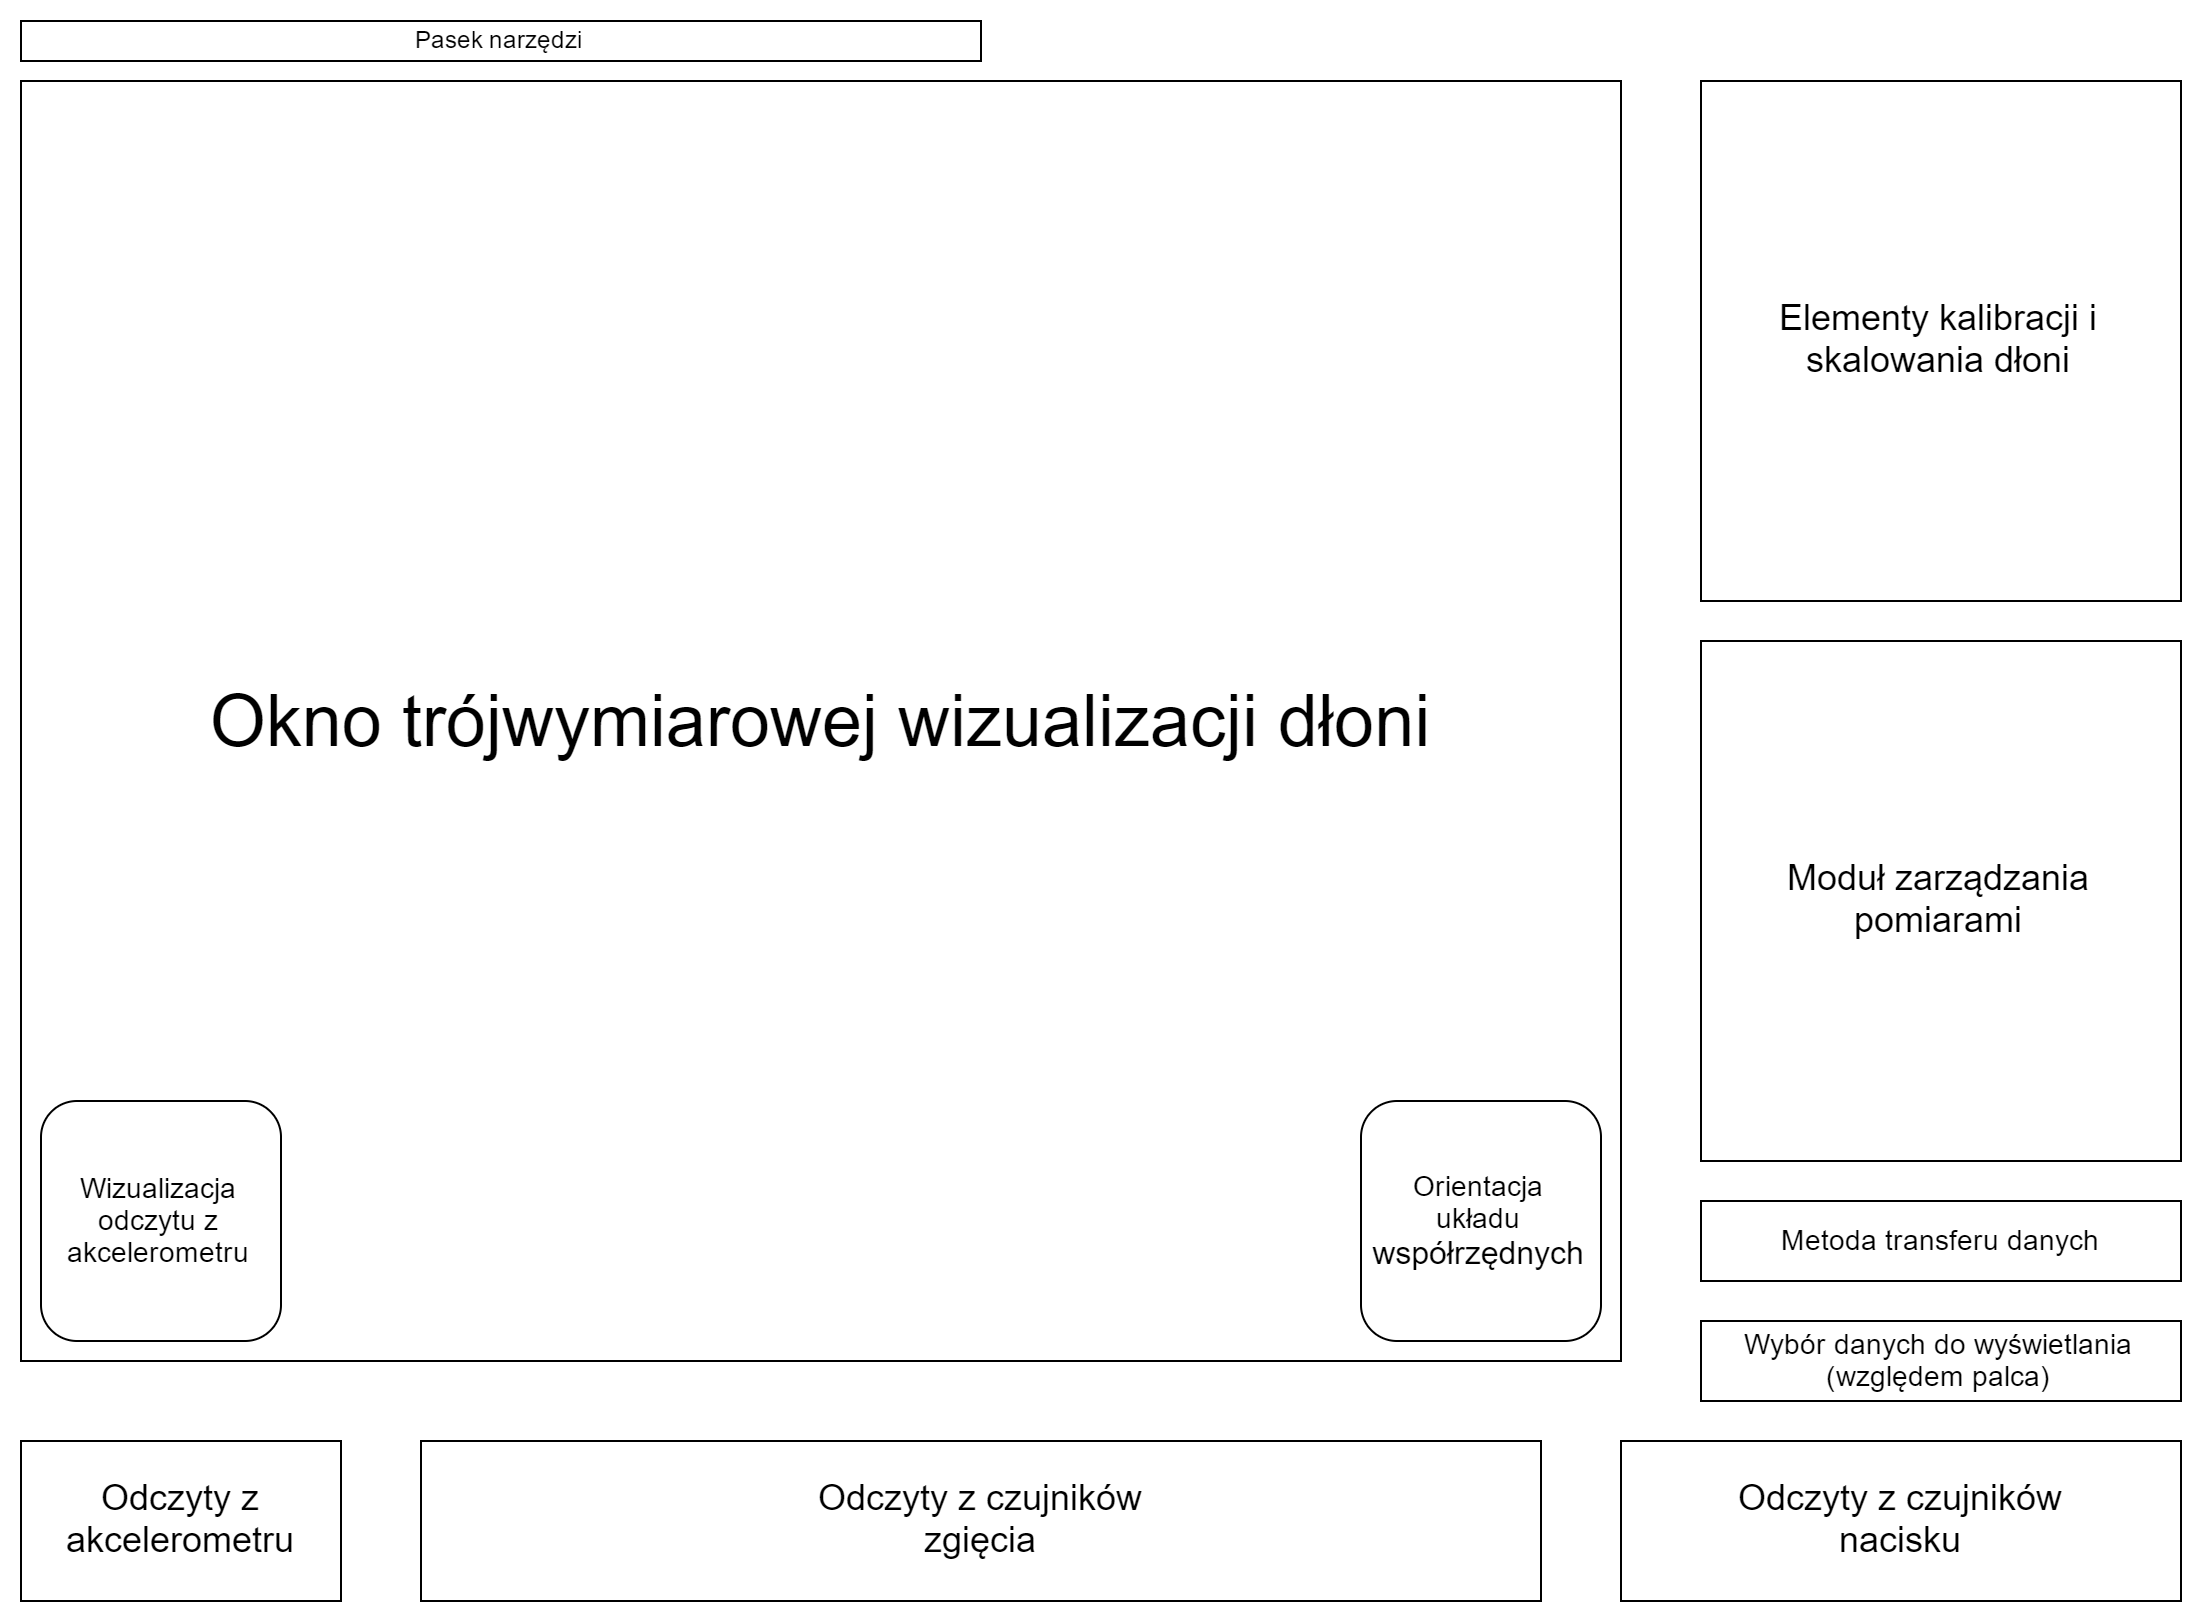
\includegraphics[width=\textwidth]{./WDS_schemat_ideowy_okna_programu.png}
\caption{Planowany interfejs graficzny aplikacji\label{fig:interface}}
\end{figure}

\newpage
\subsection{Diagramy klas}
Diagram klas przetwarzających dane i obliczeniowych w aplikacji, przedstawiony na rysunku \ref{fig:classdiagram} wykonany został w języku UML.\\
\begin{figure}[!htb]
\centering
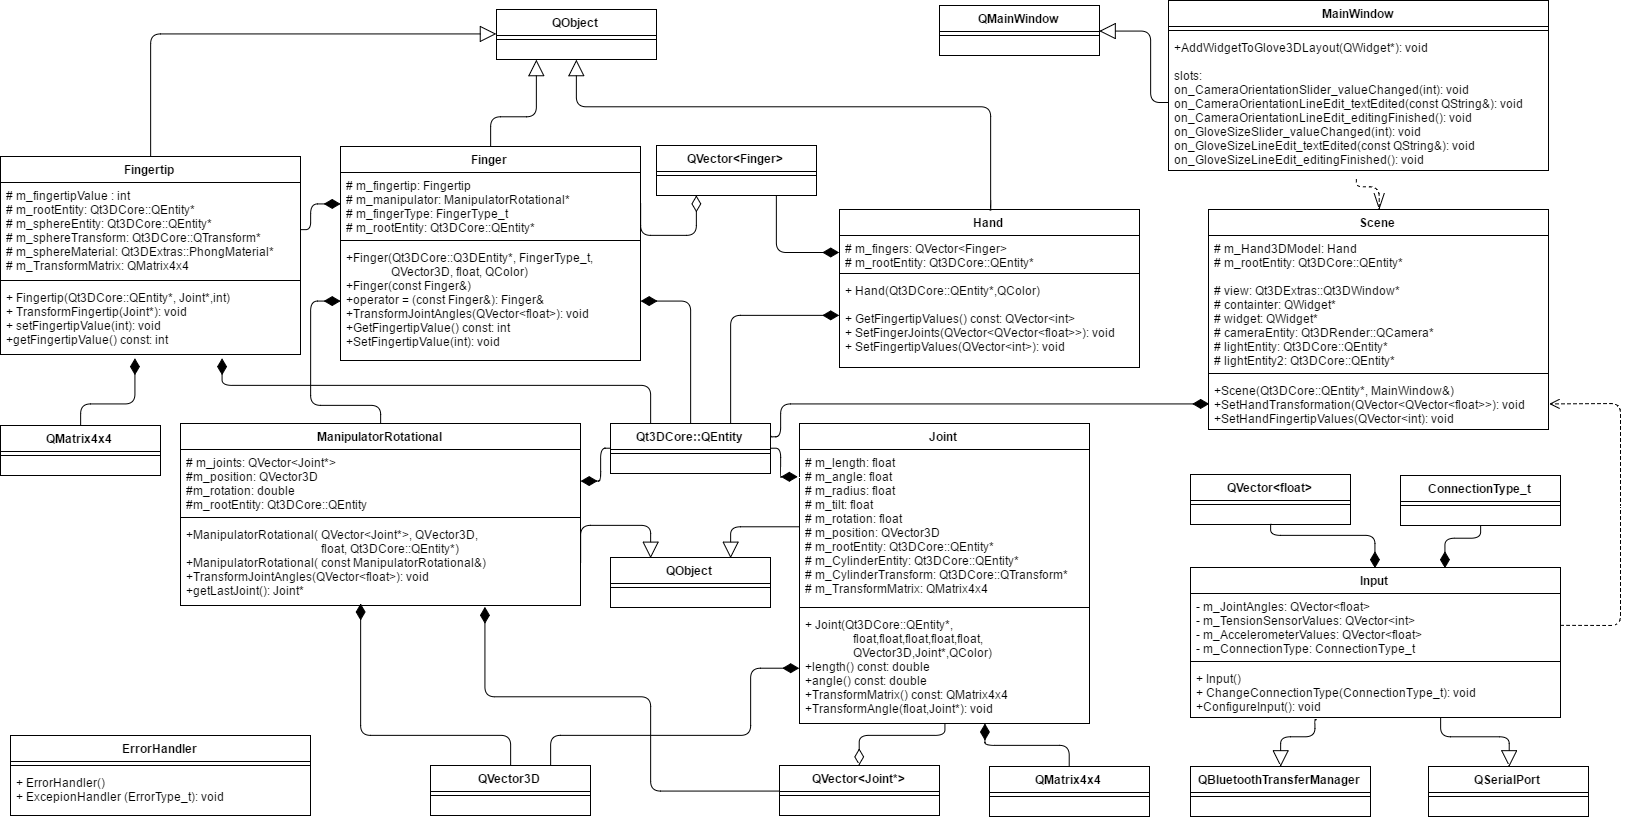
\includegraphics[angle=90,height=0.8\textheight]{./ClassDiagram.png}
\caption{Diagram klas części aplikacji odpowiedzialnej za przetwarzanie danych\label{fig:classdiagram}}
\end{figure}

\subsection{Schemat blokowy}
%DIMA!!! O TUTAJ
%TUTAJ DODAJ
%SZYBKO NIE MA CZASU
%ZEGAR TYKA
%TIK TOK
% 21:00 SIĘ ZBLIŻA!
%NAKURWIAJ!!!
%Wyrównaj na stronach po dodaniu

\section{Specyfikacja urządzenia}

\subsection{Opis ogólny}
\begin{itemize}
\item Na opuszkach palców zamontowane zostaną czujniki siły nacisku FSR-400. Spadek rezystancji przy przyłożonej sile pozwala zmierzyć siłę nacisku.
\item Do wykrycia zgięcia stawów międzypaliczkowych bliższych oraz stawu międzypaliczkowego kciuka zastosowane zostaną czujniki ugięcia - flexsensory firmy Sparkfun. Zgięcie tych sensorów powoduje wzrost rezystancji.
\item Akcelerometr LSM303DLHC, znajdujący się na płytce Discovery zostanie użyty do określenia orientacji rękawicy względem wektora grawitacji.
\item Powyższe elementy nie zapewniają bardzo precyzyjnych pomiarów, ale zostały wybrane ze względu na cenę i charakter projektu, w którym zostaną zastosowane.
\item Jako urządzenie nadawcze Bluetooth posłuży moduł HC-06 z interfejsem UART podłączony do płytki Discovery.
\end{itemize}

\subsection{Schemat układu elektronicznego}
Ideowy schemat połączeń urządzenia pomiarowego, współpracującego z aplikacją został przedstawiony na rysunku \ref{fig:ideascheme}
\begin{figure}[!htb]
\centering
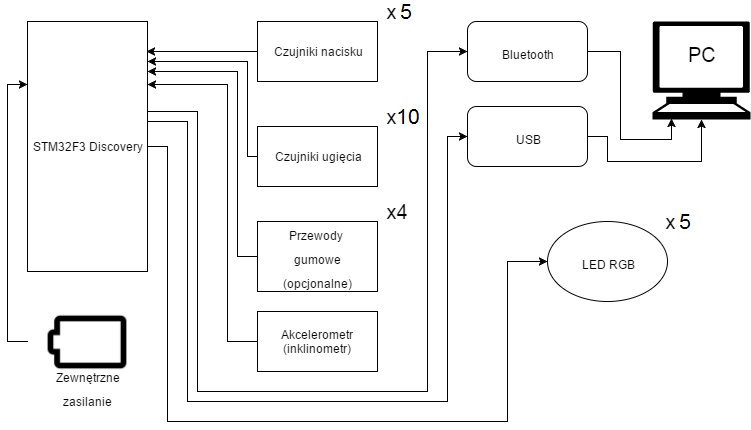
\includegraphics[width=\textwidth]{./SchematIdeowy.png}
\caption{Ideowy schemat połączeń rękawicy sensorycznej\label{fig:ideascheme}}
\end{figure}

\subsection{Parametry układu pomiarowego}
\subsubsection{Konfiguracja przetwornika pomiarowego}
\begin{itemize}
\item Rozdzielczość przetwornika: 12 bitów
\item Zakres pomiarowy: (0 - 4095: int), (0 - 3.3 V)
\item Pomiar ciągły z wykorzystaniem DMA
\item Czas próbkowania: 19.5 Cykli
\item Częstotliwość zegara: 32 MHz
\end{itemize}

\newpage
\subsubsection{Opis czujników}
\begin{itemize}
\item Na opuszkach palców zamontowane zostaną czujniki siły nacisku FSR-400. Spadek rezystancji przy przyłożonej sile pozwala zmierzyć siłę nacisku.
\item Do wykrycia zgięcia stawów międzypaliczkowych i śródręczno-paliczkowych oraz stawów kciuka zastosowane zostaną czujniki ugięcia - flexsensory firmy Sparkfun. Zgięcie tych sensorów powoduje wzrost rezystancji.
\item Akcelerometr LSM303DLHC, znajdujący się na płytce Discovery zostanie użyty do określenia orientacji rękawicy względem wektora grawitacji.
\end{itemize}
\subsubsection{Dane czujnika ugięcia}
\begin{itemize}
\item Długość powierzchni czynnej: 55.37 mm
\item Zakres rezystancji: 25 kOhm - 125 kOhm
\item Rezystor pomiarowy do dzielnika: 62 kOhm
\end{itemize}
\subsubsection{Dane czujnika nacisku}
\begin{itemize}
\item Średnica powierzchni czynnej: 5 mm
\item Zakres pomiarowy nacisku: 0.2 - 20 N
\item Zakres rezystancji: 150 Ohm - 10 MOhm
\item Rezystor pomiarowy do dzielnika: 3 kOhm
\end{itemize}
\subsubsection{Dane z akcelerometru}
\begin{itemize}
\item Protokół komunikacyjny: $I^2C$
\item Ilość osi: 3
\item Maksymalne przeciążenie: 16g
\item Dokładność pomiaru: 16 bitów 
\end{itemize}

\subsection{Opis protokołu komunikacji}
Wykorzystano dwa sposoby komunikacji z urządzeniem pomiarowym. Możliwość przełączania między urządzeniami została przewidziana w aplikacji. Część danych odbieranych z rękawicy zostanie wstępnie przetworzona przez urządzenie pomiarowe.
\subsubsection{Bluetooth}
\begin{itemize}
\item Nazwa modułu komunikacyjnego: HC-06
\item Interfejs komunikacyjny ze strony urządzenia: UART
\item Interfejs komunikacyjny ze strony aplikacji: Serial COM Port / moduł QtBluetooth
\item Baud Rate: 9600 b/s
\item Długość słowa: 8 bit
\item Parzystość: brak
\item Bity stopu: 1
\item Nadpróbkowanie: 16 próbek
\item Wykorzystanie przerwań i/lub DMA
\end{itemize}
\subsubsection{USB - Serial Port}
\begin{itemize}
\item Nazwa modułu komunikacyjnego: Wbudowany
\item Interfejs komunikacyjny ze strony urządzenia: USB Device (FS)
\item Interfejs komunikacyjny ze strony aplikacji: Serial COM Port
\item Szybkość: 12 Mb/s
\item Maksymalna wielkość pakietu: 64 B
\end{itemize}

\newpage
%Rozpisać na kolejne tygodnie
\section{Harmonogram}
\begin{itemize}
\item (31.03.2017) Uruchomienie i przetestowanie pętli USB$\rightarrow $UART$\rightarrow $USB w celu symulacji danych sensorycznych \textbf{(Wykonane)}
\item (14.04.2017) Stworzenie struktur danych wykorzystywanych w aplikacji (przeguby, manipulatory, scena) \textbf{(Wykonane)}
\item (14.04.2017) Stworzenie projektu okna programu \textbf{(Wykonane)}
\item (23.04.2017) Wczytywanie i dekodowanie danych z rękawicy sensorycznej
% Wstępne rezultaty
\item (05.05.2017) Stworzenie uproszczonego modelu kośćca dłoni
\item (05.05.2017) Stworzenie elementów potrzebnych do wizualizacji czujników (okna programu)
\item (14.05.2017) Poruszanie przegubami na podstawie odczytów z tensorów i kinematyki prostej manipulatorów
\item (14.05.2017) Zmiana koloru i/lub wielkości sfer na podstawie odczytów z czujników nacisku
%Rezultaty prawie końcowe
\item (26.05.2017) Obrót modelu na podstawie akcelerometru
\item (26.05.2017) Komunikacja przez Bluetooth
\item (02.06.2017) Testy aplikacji
\item (11.06.2017) Naprawianie błędów
\item (11.06.2017) Wizualne ulepszenie aplikacji
%Rezultaty końcowe
\end{itemize}

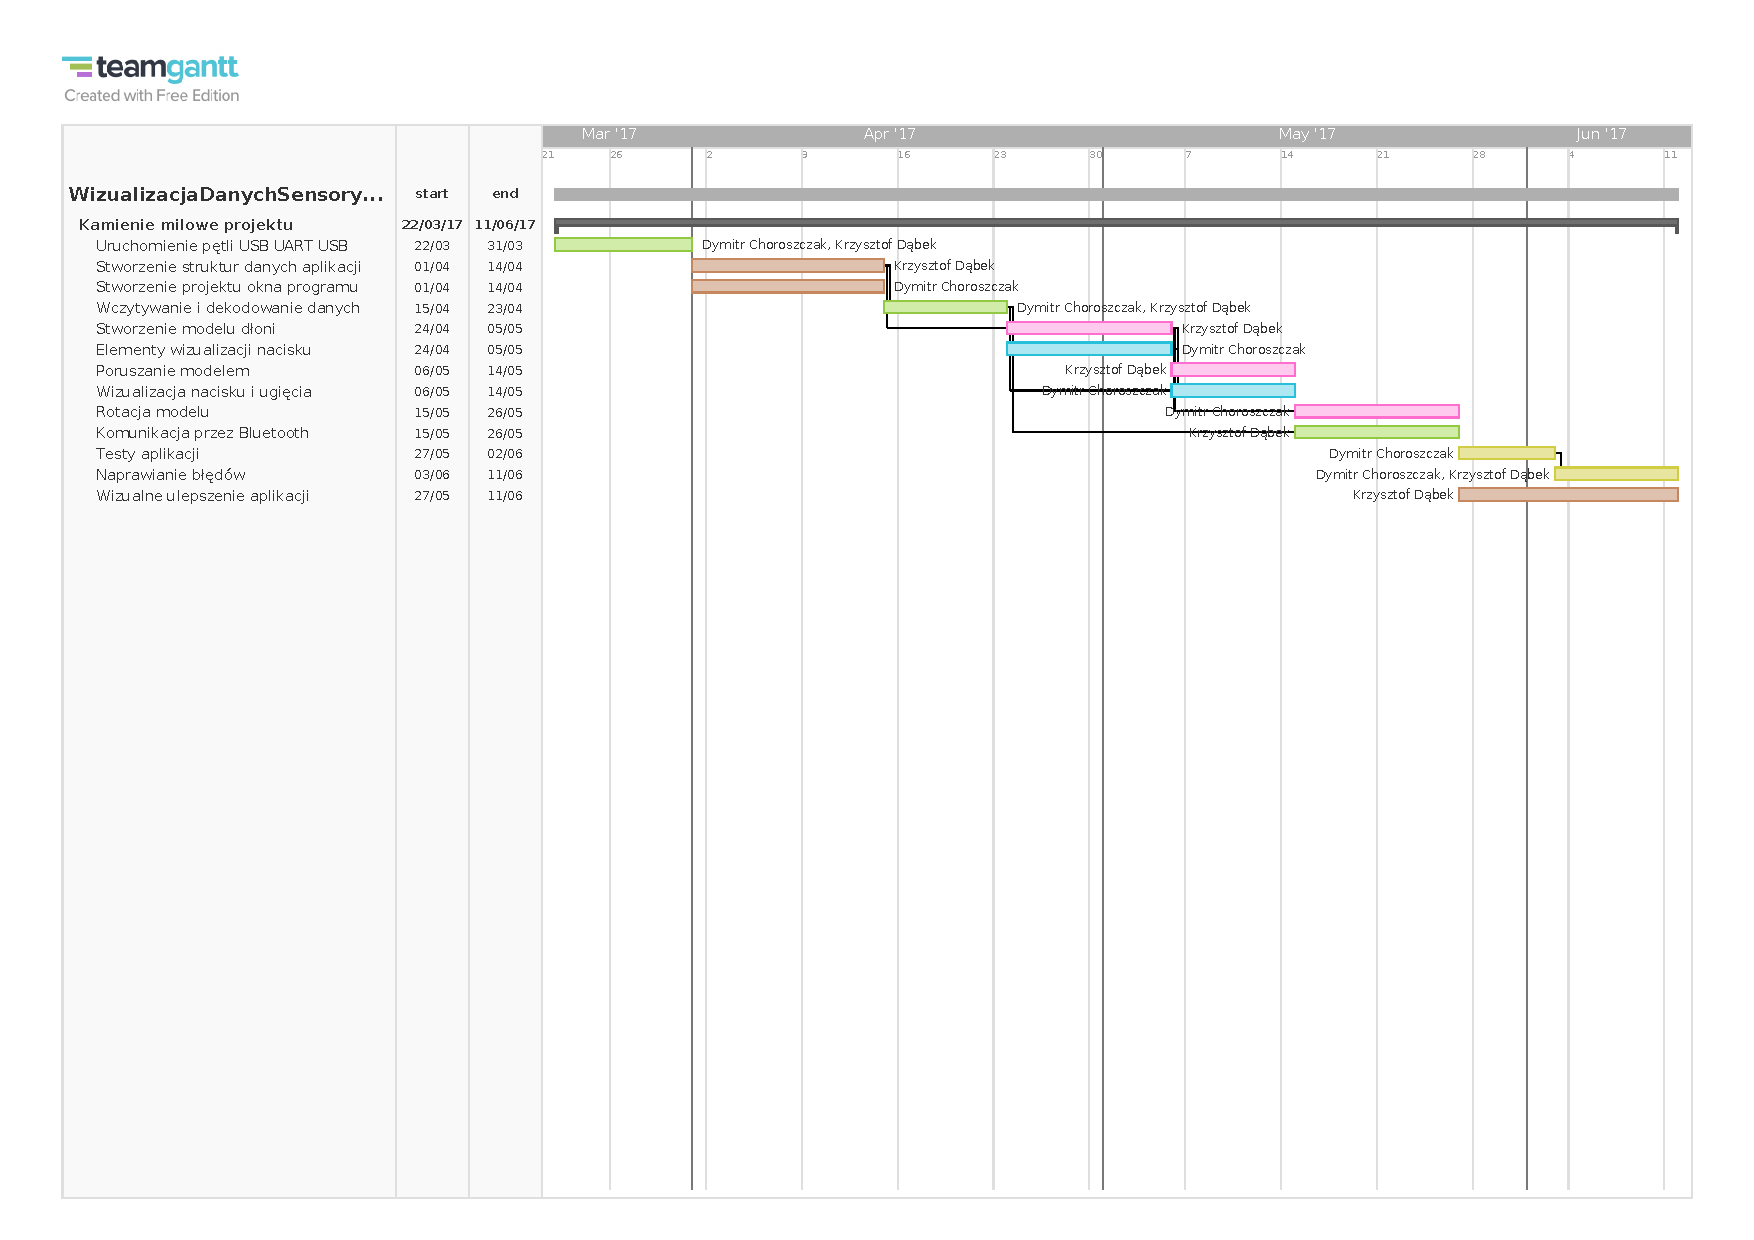
\includepdf[pages={-},angle=90]{Gantt.pdf}

\end{document}